\subsection{Diagram klas}

Zdecydowaliśmy się na wzorzec architektoniczny MVC (ang. Model View Controller). 
Jego zastosowanie umożliwia łatwą modyfikowalność, któregoś z komponentów, bez                                                                                               
konieczności zmian w pozostałych. Zgodnie z tym wzorcem w modelu zgromadzone są wszystkie dane naszego systemu. 
Widok odpowiada za prezentację aktualnego stanu systemu użytkownikowi, a kontroler odpowiada za zmianę modelu, a także odświeżanie widoków.
Na rysunku \ref{fig:mvc} przedstawiono trzy części wzorca MVC naszego systemu.

\begin{figure}[h]
    \centering
    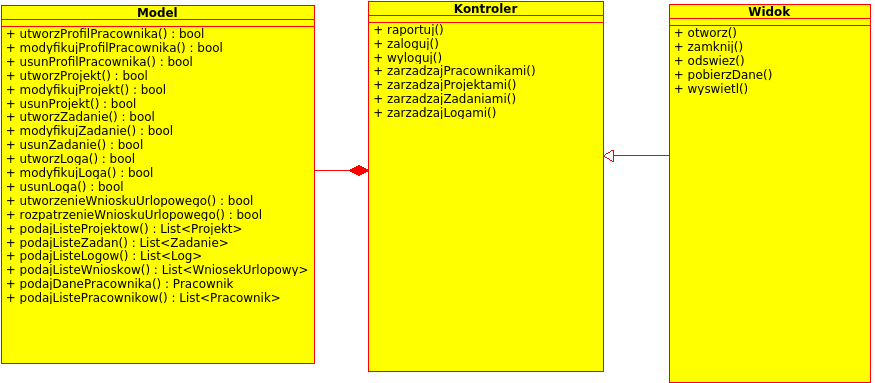
\includegraphics[scale=0.7]{modelKlas/mvc}
    \caption{Schemat architektury systemu zgodnej ze wzorcem architektonicznym MVC}
    \label{fig:mvc}
\end{figure}


